\section{Forças}
\subsection{Conteúdo Importante}
\subsubsection{Primeira Lei de Newton}

Com as Leis de Newton, começamos o estudo de como o movimento ocorre no mundo real. O estudo das causas do movimento é chamado de dinâmica ou mecânica. A relação entre força e a aceleração foi dada por Isaac Newton em suas três leis do movimento, que formam o base da física elementar. Embora a formulação da física de Newton tivesse que ser substituída mais tarde, para lidar com o movimento em velocidades comparáveis à velocidade da luz e para o movimento no escala de átomos, é aplicável a situações cotidianas e ainda é a melhor introdução para as leis fundamentais da natureza. O estudo das leis de Newton e suas implicações é muitas vezes chamada de mecânica newtoniana ou clássica.

As partículas aceleram porque sofrem ação de forças. Na ausência de forças, uma partícula não acelera, movendo-se com uma velocidade constante.

\begin{definition}[Primeira Lei de Newton.] Considerando um corpo no qual não hã ação de forças. Então, se esse mesmo corpo estiver em repouso, permanecerá em repouso, e se estiver se movendo com velocidade constante, continua a mover-se nessa velocidade.
\end{definition}

\subsubsection{Segunda Lei de Newton}
Experiencias demonstram que os objetos têm uma propriedade chamada \textbf{massa} que mede como o seu movimento é influenciado por forças. A Segunda Lei de Newton é uma relação entre a \textbf{força resultante} ($F$) agindo sobre uma massa $m$ e sua aceleração $a$.

\begin{definition}[Segunda Lei de Newton] $\sum F=ma$
\end{definition}

A relação acima é uma relação \emph{vetorial}, pelo que em duas dimensões, esta equação implica:

\begin{equation}\label{eqn:2newton}
    \sum F_x=ma_x \qquad \sum F_y=ma_y
\end{equation}

A unidade de força no SI é $kg\ ms^{-2}$, abreviada em newton ($N$). Deste modo,

\begin{equation*}
    1\ newton = 1 N = 1\ kg\ ms^{-2}
\end{equation*}

\subsubsection{Exemplos de Forças}
A Terra exerce uma força gravitacional com sentido para baixo em todas as massas perto da sua superfície. Esta força é conhecida como o \textbf{peso}, $F_g$, e a sua magnitude é dada por

\begin{equation}
    F_g=mg    
\end{equation}

Uma corda sob tensão exerce uma força nos objetos que estão apensos em cada uma das pontas. As forças estão direcionadas para dentro ao longo do comprimento da corda. A tensão é simbolizada pela letra $T$.

Uma superfície sólida exerce uma força em qualquer massa com a qual esteja em contacto. De modo geral, a força da superfície terá uma componente perpendicular/normal, denominada \textbf{força normal} da superfície. A superfície pode também exercer uma força paralela: a força de fricção.

\subsubsection{Terceira Lei de Newton}
Esta lei é popularmente enunciada como "lei da ação-reação", mas na verdade lida com as forças entre dois objetos.

\begin{definition}[Terceira Lei de Newton.] Considerando dois objetos A e B. A força que o objeto A exerce no objeto B é igual e oposta à força que o objeto B exerce no objeto A: $F_{AB}=-F_{BA}$
\end{definition}

\subsubsection{Aplicação das Lei de Newton}
Uma dica útil apra problemas que envolvem mais do que uma força é desenhar um diagrama que evidencia as massas individuais no problema, juntamento com os vetores que mostram as direções e magnitudes das forças individuais. A estes diagramas é dado o nome de \textbf{diagramas de corpo-livre}.

\subsubsection{Atrito}
Forças que são conhecidas coletivamente como “forças de atrito” estão ao nosso redor na vida diária. Na física elementar, discutimos a força de atrito conforme ela ocorre entre dois objetos cujas
superfícies estão em contato e deslizam uma contra a outra. Se, em tal situação, um corpo não se mover enquanto uma força $F$ age sobre ele, então
as forças de \textbf{atrito estático} opõem-se à força $F$, pelo que a força resultante será zero. Empiricamente,
descobre-se que esta força pode ter um valor máximo dado por:

$$
f_s^{max}=\mu_sN
$$

onde $\mu_s$ é o \textbf{coeficiente de atrito estático} para as duas superfícies e $N$ é a força normal entre as duas.
Se um objeto está em movimento em relação a outro, então existe uma força de \textbf{atrito cinético} entre os dois objetos. A direção desta força é tal que se opõe ao movimento e a sua magnitude é dada por

$$
f_k=\mu_kN
$$

onde $N$ é a força normal entre os objetos e $\mu_k$ o \textbf{coeficiente de atrito cinético} para as duas superfícies.

\subsubsection{Revisitando o Movimento Circular Uniforme}

Como visto em capítulos anteriores, quand oum objeto está em movimento circular uniforme, movendo-se em forma de círculo de raio \emph{r} com velocidade \emph{v}, a aceleração (centrípeta) é dirigida para o centro do círculo e tem magnitude

\begin{equation}
    a_{c}=\frac{v^2}{r}
\end{equation}

Desta maneira, da Segunda Lei de Newton, a força resultante que atua neste objeto tem também de ser direcionada para o centro da trajetória e ter magnitude

\begin{equation}
    F_{c}=\frac{mv^2}{r}
\end{equation}

Tal força é chamada \textbf{força centrípeta}.

\subsubsection{Lei da Gravitação Universal}
A força gravítica é uma das forças fundamentais da natureza. Todas as massas exercem uma força gravitacional atrativa umas sobre as outras, mas para a maioria dos objetos a força é tão pequena que podemos ignorá-la.

A Lei da Gravitação Universal diz que para duas massas $m_1$ e $m_2$, separadas por uma distância $r$, a magnitude da força gravitacional é

\begin{equation}\label{eq:lei_da_gravidade}
    F=G\frac{m_1m_2}{r^2} \qquad onde \qquad G=6.67\times 10^{-11}\frac{N\cdot m^2}{kg^2}
\end{equation}

% \section{Exercícios}
% \subsection{Segunda Lei de Newton}
\textbf{1.} Uma massa de 3.0kg sofre uma aceleração dada por $a=(2.0i + 5.0j)ms^{-2}$. Qual é a força resultante e a sua magnitude?
\linebreak
A Segunda Lei de Newton diz-se que a força resultante numa massa $m$ é $\sum F = ma$. Portanto,

$$
\begin{aligned}
    F_{R}&=ma \\
        &=(3.0\ kg)(2.0i+5.0j)ms^{-2} \\
        &=(6.0i + 15j)N
\end{aligned}
$$

A magnitude da $F_{R}$ é dada pelo cálculo da norma do vetor $F_{R}$:

$$
\begin{aligned}
    F_{R}=\sqrt{(6.0N)^2+(15.0N)^2}=16N
\end{aligned}
$$

\textbf{2.} Enquanto duas forças agem sobre ela, uma massa de $m=3.2kg$ move-se com uma velocidade constante $(3ms)i-(4ms)j$. Uma dessas forças é $F_1=(2N)i+(-6N)j$. Qual é a outra força?
\linebreak
A Segunda Lei de Newton diz-se que a força resultante numa massa $m$ é $\sum F = ma$. Portanto, $\sum F = ma \equiv F_1+F_2=ma$. Neste caso, a velocidade é constante, pelo que $a=0$. Portanto,

$$
\begin{aligned}
    F_1+F_2&=0 \\
    \implies F_2&=-F_1 \\
    \implies F_2&=-[(2N)i+(-6N)j] \\
    \implies F_2&=(-2N)i+(6N)j
\end{aligned}
$$

\textbf{3.} Um objeto de massa $m=4.0\ kg$ tem uma velocidade de $3.0i\ ms^{-1}$ num dado instante. Oito segundos depois, a sua velocidade é $(8.0i+10.0j)ms^{-1}$. Assumindo que o objeto foi sujeito a uma força resultante constante, encontre (a) as componentes da força e (b) a sua magnitude. \\
\linebreak
\textbf{(a)} É-nos dito que a força resultante que age na massa foi constante. Logo, sabemos que a sua aceleração foi igualmente constante, we podemos usar resultados de capítulos anteriores. São facultadas as velocidades inicias e final, pelo que é possível calcular as componentes da aceleração:

$$
a_x=\frac{\Delta v_x}{\Delta t}=\frac{[(8.0\ ms^{-1})-(3.0\ ms^{-1})]}{(8.0\ s)}=0.63\ ms^{-2}
$$

$$
a_y=\frac{\Delta v_y}{\Delta t}=\frac{[(1.0\ ms^{-1})-(0.0\ ms^{-1})]}{(8.0\ s)}=1.3\ ms^{-2}
$$

Visto que a massa é facultada no enunciado, é possível calcular as componentes da força resultante:

$$
\begin{aligned}
    F_x=ma_x=(4.0\ kg)(0.63\ ms^{-2})=2.5N \\
    F_y=ma_y=(4.0\ kg)(1.3\ ms^{-2})=5.0N \\
\end{aligned}
$$

\textbf{(b)} A magnitude da força resultante é obtida através da seguinte computação:

$$
F=\sqrt{F_x^2+F_y^2}=\sqrt{(2.5\ N)^2+(5.0\ N)^2}=5.6\ N
$$

A direção $\theta$ da força $F$ é dada por

$$
\tan \theta = \frac{F_y}{F_x} = 2.0 \quad \implies \quad \theta = \arctan(2.0)=63.4^{\circ}
$$

\textbf{4.} Cinco forças atuam sobre a caixa de massa $4.0\ kg$ na Figura \ref{fig:4caixa}. Encontre a aceleração da caixa (a) na notação unidade-vetor e (b) a sua magnitude e direção.
\linebreak
\begin{figure}[h!]
    \centering
    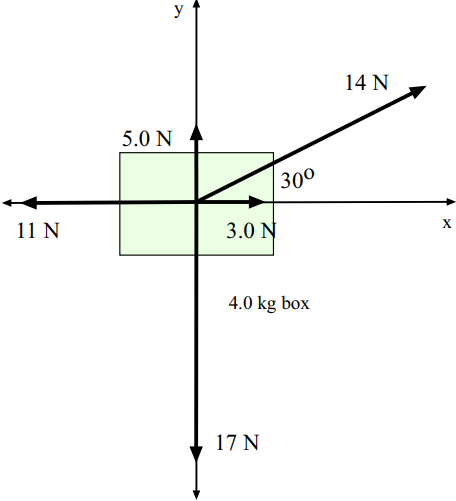
\includegraphics[width=0.5\textwidth]{forças/fig/ex4.png}
    \caption{Cinco forças atuam num caixa de massa $4.0\ kg$.}
    \label{fig:4caixa}
\end{figure}


\textbf{(a)} Existe a necessidade de separar as forças nas suas duas componentes $x$ e $y$. A Segunda Lei de Newton será utilizada para computar o valor da aceleração da caixa.

$$
\begin{aligned}
    \sum F_x&=-11N+3N+14\cos(30º) \\
    &=4.1N
\end{aligned}
$$

$$
\begin{aligned}
    \sum F_y&=+5N-17N+14\sin(30) \\
    &=-5.0N
\end{aligned}
$$

Logo, tem-se que a força resultante é

$$
\sum F=(4.1N)i+(-5.0N)j
$$

Utilizando a Equação \ref{eqn:2newton}, temos:

$$
    \sum a_x=\frac{\sum F_x}{m}=\frac{(4.1\ N)}{4.0\ kg}=1.0\ ms^{-2} \\
    \sum a_y=\frac{\sum F_y}{m}=\frac{(-5.0\ N)}{4.0\ kg}=-1.2\ ms^{-2} \\
$$


O valor da aceleração em notação vetorial é, então,

$$
a=(1.0i-1.2j)ms^{-2}
$$

\textbf{(b)} A aceleração encontrada em (a) tem magnitude

$$
a=\sqrt{a_x^2+x_y^2}=\sqrt{(4.0\ ms^{-2})^2+(-1.2\ ms^{-2})^2}=1.6\ ms^{-2}
$$

A direção $\theta$ do vetor aceleração é dada por

$$
\tan \theta = \frac{a_y}{a_x} = -1.2 \quad \implies \quad \theta = \arctan(-1.2)=-50^{\circ}
$$

Neste caso, tendo em conta que $a_y$ é negativo e $a_x$ é positivo, a escolha de $\theta = -50^{\circ}$ está correta.

\subsection{Exemplos de Forças}
\textbf{5.} Encontre a tensão em cada uma das cordas da Figura \ref{fig:5caixa}.
\linebreak
\begin{figure}[h!]
    \centering
    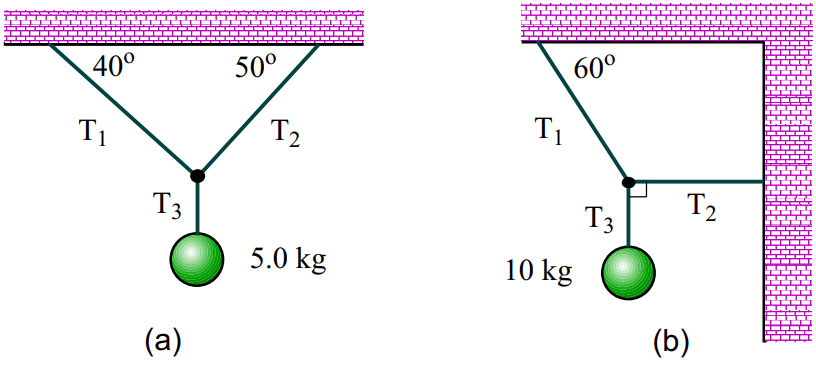
\includegraphics[width=0.5\textwidth]{forças/fig/ex5.png}
    \caption{Massas suspensas por cordas.}
    \label{fig:5caixa}
\end{figure}

\textbf{(a)} Seja $m_1$ a massa correspondente à bola representada na Figura \ref{fig:5caixa} (a). A força gravítica atua para baixo com uma força de magnitude $m_1g$. A corda vertical puxa "para cima" com uma força de magnitude $T_3$. Tendo em conta que a massa pendurada não tem aceleração, verifica-se que $T_3=m_1g$. Portanto, o valor de $T_3$ é dado por:

$$
T_3=m_1g=(5.0\ kg)(9.9\ ms^{-2})=49\ N
$$

Considerando agora o ponto de união das três cordas. Esse ponto não tem qualquer aceleração, pelo que o resultado da força resultante deverá ser zero. As componentes verticais e horizontains dessas forças somam a zero, separadamente.

$$
    \begin{cases}
        -T_1\cos(40^{\circ})+T_2\cos(50^{\circ})=0 \\
        T_1\sin(40^{\circ})+T_2\sin(50^{\circ})-T_3=0
    \end{cases}
$$

A primeira equação, a soma das componentes horizontais, dá-nos $T_2=1.19T_1$.

A segunda equação,  a soma das componentes verticais, dá-nos o valor  $T_1=31.5\ N$.

Sabendo o valor de $T_1$, $T_2=1.19T_1\ \implies \ T_2=37.5\ N$

As tensões no sistema (a) são, portanto:

$$
T_1=31.5\ N \qquad T_2=37.5\ N \qquad T_3=49\ N
$$

\textbf{(b)} A força resultante na massa pendurada, $m_2$, tem de ser 0, porque não há aceleração. Visto que a gravida "puxa para baixo" com uma força $m_2g$ e a corda vertical "puxa para cima" com uma força $T_3$, sabemos que

$$
T_3-F_g=0 \implies T_3=F_g \implies T_3=m_2g \\
\begin{aligned}
    T_3&=m_2g
    &=(10\ kg)\cdot(9.8\ ms^{-2})=98\ N
\end{aligned}
$$

Considerando agora as forças que atuam no ponto onde todas as forças se encontram. Novamente, como não há aceleração nesse ponto, tanto as componentes verticais como horizontais somam a zero.

No que toca às forças horizontais, temos:

$$
-T_1\cos(60^{\circ})+T_2=0 \qquad \implies \qquad T_2=T_1\cos(60^{\circ}) \\
$$

A soma das forças verticais é dada por:

$$
T_1\sin(60^{\circ})-T_3=0 \qquad \implies \qquad T_1=\frac{T_3}{\sin(60^{\circ})}=113\ N
$$

Podemos, depois, obter $T_2$:

$$
T_2=T_1\cos(60^{\circ})=(133\ N)\cos(60^{\circ})=56.6\ N
$$

As tensões no sistema (b) são, portanto:

$$
T_1=133\ N \qquad T_2=56.6\ N \qquad T_3=98\ N
$$

\textbf{6.} Um bloco de massa $m=2.0\ kg$ está suspenso em equilíbrio num encosta que faz um ângulo $\theta=60^{\circ}$ pela força horizontal $F$, como mostrado na Figura \ref{fig:6plano}. (a) Determine o valor de $F$, a magnitude de $F$. (b) Determine a força normal exercida pelo plano inclinado no bloco (ignore o atrito).
\linebreak
\begin{figure}[h!]
    \centering
    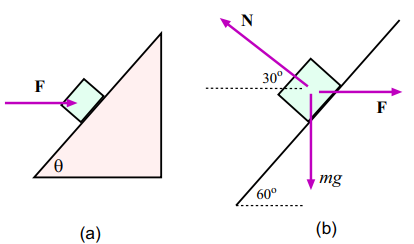
\includegraphics[width=0.5\textwidth]{forças/fig/ex6.png}
    \caption{(a) Bloco em repouso numa rampa sem atrito por uma força horizontal. (b) Forças a atuarem no bloco.)}
    \label{fig:6plano}
\end{figure}

\textbf{(a)} Fazer um diagrama de das forças que atuam no corpo torna-se essencial para este problema, daí a inclusão da \ref{fig:6plano} (b). Muitas vezes, para problemas envolvendo um bloco num plano inclinado, é mais fácil usar as componentes da $F_g$ ao longo desse mesmo plano inclinado e perpendicular a ele. Para este problema, isso não torna as coisas mais fáceis, uma vez que não há movimento no plano inclinado.

Do enunciado, retira-se a informação de que o block está em equilíbrio, pelo que não tem aceleração e as forças que em si atuam somam a zero. Este facto permite-nos escrever:

$$
N\sin(30^{\circ})-F_g=0 \qquad \implies \qquad N=\frac{F_g}{\sin(30^{\circ})}
$$

$$
N=\frac{(2.0\ kg)\cdot(9.8\ ms^{-2})}{\sin(30^{\circ})}=39.2\ N
$$

O resultado da força resultante horizontal também é nulo, logo podemos escrever:

$$
F-N\cos(30^{\circ})=0 \qquad \implies \qquad F=N\cos(30^{\circ})=33.9\ N
$$

\textbf{(b)} O resultado da força Normal foi encontrado anteriormente, $N=39.2\ N$.